\documentclass[spanish,A4,]{article}
\usepackage{sans}
\usepackage{amssymb,amsmath}
\usepackage{ifxetex,ifluatex}
\usepackage{fixltx2e} % provides \textsubscript
\ifnum 0\ifxetex 1\fi\ifluatex 1\fi=0 % if pdftex
  \usepackage[T1]{fontenc}
  \usepackage[utf8]{inputenc}
\else % if luatex or xelatex
  \ifxetex
    \usepackage{mathspec}
    \usepackage{xltxtra,xunicode}
  \else
    \usepackage{fontspec}
  \fi
  \defaultfontfeatures{Mapping=tex-text,Scale=MatchLowercase}
  \newcommand{\euro}{€}
\fi
% use upquote if available, for straight quotes in verbatim environments
\IfFileExists{upquote.sty}{\usepackage{upquote}}{}
% use microtype if available
\IfFileExists{microtype.sty}{\usepackage{microtype}}{}
\usepackage{longtable,booktabs}
\usepackage{graphicx}
\makeatletter
\def\maxwidth{\ifdim\Gin@nat@width>\linewidth\linewidth\else\Gin@nat@width\fi}
\def\maxheight{\ifdim\Gin@nat@height>\textheight\textheight\else\Gin@nat@height\fi}
\makeatother
% Scale images if necessary, so that they will not overflow the page
% margins by default, and it is still possible to overwrite the defaults
% using explicit options in \includegraphics[width, height, ...]{}
\setkeys{Gin}{width=\maxwidth,height=\maxheight,keepaspectratio}
\ifxetex
  \usepackage[setpagesize=false, % page size defined by xetex
              unicode=false, % unicode breaks when used with xetex
              xetex]{hyperref}
\else
  \usepackage[unicode=true]{hyperref}
\fi
\hypersetup{breaklinks=true,
            bookmarks=true,
            pdfauthor={},
            pdftitle={},
            colorlinks=true,
            citecolor=blue,
            urlcolor=blue,
            linkcolor=magenta,
            pdfborder={0 0 0}}
\urlstyle{same}  % don't use monospace font for urls
\setlength{\parindent}{0pt}
\setlength{\parskip}{6pt plus 2pt minus 1pt}
\setlength{\emergencystretch}{3em}  % prevent overfull lines
\setcounter{secnumdepth}{0}
\ifxetex
  \usepackage{polyglossia}
  \setmainlanguage{spanish}
\else
  \usepackage[spanish]{babel}
\fi


\begin{document}

\section{Redes de computadoras}\label{redes-de-computadoras}

Un conjunto de computadoras conectadas para compartir información u
otros recursos es una \textbf{red} de computadoras. En cualquier red se
distinguen por lo menos tres elementos de hardware:

\begin{itemize}
\itemsep1pt\parskip0pt\parsep0pt
\item
  Las computadoras conectadas se llaman \textbf{hosts} o nodos
  terminales.
\item
  Los \textbf{enlaces} que conectan las computadoras. Los enlaces suelen
  llamarse \textbf{punto a punto} cuando conectan únicamente dos nodos,
  o \textbf{compartidos} cuando al mismo enlace se conectan más de dos
  nodos.
\item
  Otros \textbf{nodos intermedios}, los \textbf{routers}, que sirven
  para encaminar el tráfico de información entre los nodos terminales.
\end{itemize}

Para utilizar la red, todos los nodos que están conectados a ella, ya
sean terminales o intermedios, corren software de red como
\textbf{protocolos} y \textbf{aplicaciones de red}. Los protocolos son,
por un lado, convenciones que establecen con todo detalle cómo se
realiza una comunicación, y por otro lado, los componentes de software
que implementan esa forma de comunicación.

Las aplicaciones de red son aplicaciones \textbf{distribuidas}, es
decir, se componen de al menos dos partes, preparadas para comunicarse
unas con otras, y esas partes funcionan en nodos terminales de la red
diferentes. Cada aplicación de red utiliza un protocolo, porque la
interacción entre las partes debe estar perfectamente determinada para
que los nodos se entiendan sin errores ni ambigüedades. Un protocolo
puede ser utilizado por varias aplicaciones.

Hoy, la mayoría de las redes están interconectadas por una única red
global llamada \textbf{Internet}. Para conectarse a Internet, todos los
nodos, terminales e intermedios, ejecutan un protocolo básico llamado
\textbf{IP (Internet Protocol)}, y se puede decir que, desde el punto de
vista del software, constituyen una sola red.

Sin embargo, desde el punto de vista de la administración, dentro de
Internet existen numerosas redes. Cada red es propiedad de una persona u
organización que tiene el control sobre los nodos y enlaces de esa red,
decide qué nodos pertenecen o no pertenecen a ella, y qué protocolos y
aplicaciones utilizan.

Estas diferentes redes se pueden clasificar por su tamaño.

\begin{itemize}
\itemsep1pt\parskip0pt\parsep0pt
\item
  Una red cuyos límites (o \textbf{diámetro}) son pequeños, se llama una
  \textbf{red de área local o LAN (Local Area Network)}. Típicamente,
  una LAN está contenida en una oficina, piso o edificio.
\item
  Una red que abarca el área de una ciudad (y por lo tanto, cuyos
  enlaces utilizan espacios públicos) suele llamarse \textbf{red
  metropolitana o MAN (Metropolitan Area Network)}.
\item
  Una red mayor, que cubre distancias entre ciudades, países o
  continentes, se llama una \textbf{red de área extensa o WAN (Wide Area
  Network)}. Las redes de los \textbf{proveedores de servicios de
  Internet (ISPs)} suelen clasificarse como WANs.
\end{itemize}

\subsection{Modelo de Internet}\label{modelo-de-internet}

Las redes pueden estudiarse y comprenderse mediante modelos jerárquicos
compuestos por capas, donde cada pieza de hardware o de software
pertenece a una capa o nivel.

Cada capa corresponde a un conjunto de problemas relacionados, y a las
soluciones posibles. Para funcionar, cada capa se apoya en las
soluciones provistas por la capa inmediatamente inferior.

\begin{itemize}
\item
  Aplicación

  En la capa de Aplicación se encuentran los protocolos sobre los cuales
  se basan directamente las aplicaciones distribuidas.
\item
  Transporte

  La capa de Transporte soluciona el problema de la entrega de datos
  entre \textbf{procesos} de nodos diferentes.
\item
  Red

  La capa de Red soluciona el problema de la entrega de datos entre
  \textbf{nodos} de diferentes redes.
\item
  Enlace

  La capa de Enlace soluciona el problema de la entrega de datos entre
  \textbf{nodos de la misma red}.
\item
  Física

  La capa Física define la forma como se codifican y transmiten las
  señales que representan la información.
\end{itemize}

\subsection{Switches}\label{switches}

En las redes de área local, o LAN, encontramos enlaces compartidos. El
cableado de una oficina, un aula o un edificio es un único medio de
comunicación compartido por todos los nodos de la red. El cableado se
concentra en un punto de conmutación llamado \textbf{switch} o,
justamente, conmutador, que distribuye el tráfico entre los nodos
conectados. Un switch tiene muchas \textbf{interfaces} donde se conectan
cables punto a punto hacia los nodos de la LAN.

Es posible conectar switches entre sí para mejor distribución del
tráfico, formando una \textbf{topología} de estrella o de árbol. Todo el
conjunto de switches y enlaces de la LAN constituye un enlace
compartido, ya que todos los nodos de la LAN pueden comunicarse a través
de él.

Los switches y los nodos de las redes de área local ejecutan un
protocolo de enlace definido por la norma \textbf{IEEE 802.3}. Este
protocolo deriva de uno anterior, llamado \textbf{Ethernet}. Aunque el
diseño original de Ethernet era diferente del de 802.3, y el hardware
sobre el que funcionaba Ethernet era muy diferente del de los switches
actuales, este nombre de Ethernet sigue usándose informalmente para las
redes construidas con switches 802.3.

Un switch 802.3 conduce unas unidades de tráfico básicas, los
\textbf{frames o tramas} 802.3, entre los nodos de la red de área local,
conectados al enlace compartido formado por todos los switches y
cableado de la LAN. La misión de este protocolo de enlace termina donde
termina la red de área local. Los frames o tramas jamás salen fuera de
la LAN. Por eso decimos que la función de \textbf{nivel de enlace} de
una red es entregar el tráfico \textbf{entre nodos adyacentes}. Es
decir, los que se encuentran sobre el mismo enlace.

\subsection{Routers}\label{routers}

Suele definirse a Internet como ``red de redes''. Las grandes redes, y
en particular Internet, se componen interconectando redes a través de
enlaces, a veces de gran longitud. Entre cada dos de estas redes siempre
existe un \textbf{router}.

El router presta el servicio que no alcanza a prestar el nivel de
enlace, que es el de enviar el tráfico fuera de la red de origen. El
nivel al que pertenecen los routers se llama \textbf{nivel de red}.

Los routers son los elementos que toman las decisiones de
\textbf{enrutamiento} o ruteo, al determinar por cuál de sus interfaces,
que a veces son muchas, debe ser enviada la información que reciben.
Esta tarea de enrutar la información se cumple mediante software de
enrutamiento.

El hardware y el sistema operativo de los routers pueden estar altamente
especializados en la tarea de ruteo, pero también es perfectamente
posible construir un router a partir de una computadora corriente de
escritorio y un sistema operativo multipropósito. Es decir que los
routers no son sino computadoras, con un sistema operativo y un hardware
similares a los que encontramos en muchas otras computadoras, pero
dedicadas a la tarea del enrutamiento.

Dependiendo del ambiente donde deben trabajar y de la cantidad de
tráfico que deben procesar, los routers pueden adoptar muchas formas
físicas y tamaños.

\begin{itemize}
\item
  Los routers pueden ser pequeños y baratos, para uso doméstico.
\item
  Algunos pueden dar servicio a muchos nodos terminales al incluir
  múltiples dispositivos de nivel de enlace, como un switch 802.3 de
  varias interfaces, y un \textbf{punto de acceso} para una \textbf{red
  inalámbrica} secundaria basada en tecnología de radio.
\item
  Algunos, de muy altas prestaciones, usados por los proveedores de
  servicios de Internet, son \textbf{modulares} y pueden ser
  configurados a medida de las necesidades. Cada módulo contiene
  \textbf{interfaces} especializadas en alguna tecnología de enlace, lo
  que les permite conectar redes de tecnologías completamente
  diferentes.
\end{itemize}

\subsection{Interfaces}\label{interfaces}

La interfaz es el punto de conexión entre un enlace y un nodo de la red.
Es la pieza de hardware que convierte bits a señales capaces de viajar
por la red, y viceversa. Cuando un nodo debe comunicar algo a otro,
prepara su mensaje en una zona de la memoria, y entrega esos contenidos
binarios a la interfaz a través de un bus de comunicación.

La interfaz contiene el hardware necesario para traducir ese
\textbf{tren de bits} a señales eléctricas (cuando los enlaces son
cableados), de radio (cuando el enlace es inalámbrico), o luminosas
(cuando el enlace es de fibra óptica).

Las modernas interfaces de red pueden funcionar a \textbf{velocidades de
transmisión} de muchos bits por segundo. Una LAN cableada actual
funciona comúnmente en velocidades de 1 a 10 Gb/s o Gbps (gigabits por
segundo). Una LAN inalámbrica suele funcionar a una velocidad de
transmisión mucho menor (y, además, variable, dependiendo de condiciones
físicas ambientales que tienden a limitar la velocidad de transmisión).

El tren de bits viaja en forma de señales físicas por el enlace hasta
llegar a la interfaz del nodo destino dentro de la red de área local. La
interfaz receptora decodifica las señales, recuperando los bits
originales y comunicándolos al software que espera los datos. Ambas
partes de la aplicación distribuida se han comunicado un mensaje.

\subsection{Medios y enlaces}\label{medios-y-enlaces}

El material que atraviesan las señales transmitidas sobre un enlace se
llama el \textbf{medio} del enlace. Las tecnologías de construcción de
los enlaces son muchas.

\begin{itemize}
\itemsep1pt\parskip0pt\parsep0pt
\item
  Cuando las señales se codifican mediante impulsos eléctricos, como en
  las redes de cables de \textbf{par trenzado} o \textbf{coaxial}, el
  medio es un conductor, como el cobre.
\item
  Para distancias mayores (como las transoceánicas) o para ambientes
  donde existe mucho \textbf{ruido} o interferencia electromagnética
  (como en fábricas), se utiliza \textbf{fibra óptica}.
\item
  Cuando no es posible, o práctico, tender un cable, no queda más
  solución que utilizar emisiones de \textbf{radio}. Ejemplos de
  tecnologías de radio son los enlaces satelitales, los de microondas, y
  las LAN inalámbricas bajo norma \textbf{802.11} conocidas popularmente
  como \textbf{WiFi}. Estas tecnologías utilizan como medio el
  \textbf{espacio}.
\end{itemize}

Las principales compañías de conectividad del mundo tienden enlaces de
fibra óptica transoceánicos. Como la instalación de estos cables es una
maniobra muy compleja y tiene un costo altísimo, se aseguran de instalar
capacidad de transmisión en abundancia. Por ejemplo, uno de estos
enlaces tiene una capacidad de 3.2 Tbps, lo que permitiría transmitir el
contenido completo de un disco rígido de 1 TB en menos de tres segundos.
Esta capacidad es compartida entre varios proveedores de Internet que
compran el servicio de transporte.

\textbf{Interesante}

\href{http://www.submarinecablemap.com/\#/landing-point/las-toninas-argentina}{Submarine
Cable Map}

En el pasado también se usaron los enlaces satelitales para resolver el
problema de cubrir grandes distancias. Los satélites son repetidores de
radio colocados en órbita. Reciben emisiones de una estación terrena y
la comunican a otra distante, superando el problema de la curvatura
terrestre, que no permitiría la propagación en línea recta de la emisión
de radio.

Su principal inconveniente es la alta \textbf{latencia o retardo} en la
llegada de la señal desde un punto a otro, debido a las grandes
distancias que se deben enlazar. Los satélites \textbf{geoestacionarios}
o de órbita alta (\textbf{GEO}) se instalan a una altura de alrededor de
35700 km. Al ubicarlos a esta altura se alcanza un equilibrio entre la
fuerza de gravedad terrestre y la fuerza centrífuga del satélite, lo que
garantiza que permanecerán inmóviles respecto de algún punto de la
superficie terrestre, y así cubrirán siempre la misma región del
planeta. Pero la órbita alta implica una gran distancia a recorrer para
las señales, lo que introduce demoras de alrededor de un cuarto de
segundo entre estaciones terrestres. Estas demoras son tolerables para
algunas aplicaciones de tráfico de datos, pero perjudiciales para las
comunicaciones interactivas.

Paulatinamente van siendo abandonados en favor de la fibra óptica para
comunicación de datos a grandes distancias. Hoy se estima que sólo un
5\% del tráfico internacional es satelital, y el resto es conducido por
fibras ópticas. Sin embargo, siguen siendo una buena solución para
atravesar áreas continentales, o para distribuir tráfico hacia muchos
puntos simultáneos de bajada, como en los medios de comunicación
televisivos (aplicación llamada \textbf{broadcasting}).

\subsection{Velocidades de transmisión y de
propagación}\label{velocidades-de-transmisiuxf3n-y-de-propagaciuxf3n}

Cada interfaz funciona a una determinada \textbf{velocidad de
transmisión}, que es la cantidad de bits por segundo que es capaz de
escribir en el enlace, o leer del enlace. Las unidades utilizadas para
expresar la velocidad de transmisión son las del sistema decimal. Así,
una medida habitual es el Gbps o gigabit por segundo ($10 elevado a la 9 b/s$). La
velocidad de transmisión suele ser llamada también \textbf{ancho de
banda digital}.

Por otro lado, una vez que \textbf{cada bit} ha sido escrito en un
enlace, ese bit aún debe viajar desde la interfaz de salida hasta la
interfaz del otro extremo del enlace. Ese viaje, aunque se realiza a
velocidades cercanas a la de la luz, \textbf{no es instantáneo}.
Dependiendo del medio, la \textbf{velocidad de propagación} de un bit
puede ser de alrededor de un 60\% a 90\% de la velocidad de la luz, que
es de unos 300.0 0 0 km/s, o $3 por  10 elevado a la 8 m/s$.

\begin{itemize}
\itemsep1pt\parskip0pt\parsep0pt
\item
  Notemos que la \textbf{velocidad de transmisión} depende
  exclusivamente de las características tecnológicas de la interfaz. Son
  la construcción y la configuración de la interfaz las que definen la
  velocidad de transmisión a la cual funcionará un enlace, y no el medio
  con el que se implementa el enlace.
\item
  Por el contrario, notemos también que la \textbf{velocidad de
  propagación} es una cuestión puramente física y \textbf{no depende de
  la tecnología de las interfaces}.
\end{itemize}

La velocidad de \textbf{transmisión} puede mejorarse si se mejoran las
tecnologías de interfaz en los extremos del enlace. Pero un medio tiene
una determinada velocidad de \textbf{propagación}, y ningún cambio en la
tecnologia de las interfaces cambiará esa velocidad.

\subsection{Tiempo de transferencia de un
mensaje}\label{tiempo-de-transferencia-de-un-mensaje}

Conocer las velocidades de transmisión y de propagación nos permite
definir un modelo para el \textbf{tiempo de transferencia} de un mensaje
a través de un enlace.

Este modelo dependerá de otras dos variables: por un lado, como es
lógico, del \textbf{tamaño} del mensaje que se quiere transmitir; y por
otro lado, de la \textbf{distancia} que separa las interfaces.

Supongamos que:

\begin{itemize}
\itemsep1pt\parskip0pt\parsep0pt
\item
  La velocidad de transmisión de la interfaz es $V$ sub transm $$.
\item
  La velocidad de propagación del medio es $V$ sub prop $$.
\item
  El mensaje es de $L$ bits.
\item
  La distancia entre interfaces, o longitud del enlace, es $D$.
\end{itemize}

Entonces:

\begin{itemize}
\itemsep1pt\parskip0pt\parsep0pt
\item
  El \textbf{tiempo de transmisión} para los $L$ bits será
  $T$ sub transm $ = L / V$ sub transm $$.
\item
  El \textbf{tiempo de propagación} para el enlace de $D$ m será
  $T$ sub prop $ = D / V$ sub prop $$.
\end{itemize}

Notemos una vez más que el \textbf{tiempo de transmisión es dependiente
de la velocidad de transmisión de las interfaces}, y no de la longitud
del enlace. Y además, que el \textbf{tiempo de propagación es función de
la longitud del enlace}, y no de la velocidad de transmisión de las
interfaces.

El \textbf{tiempo de transferencia} que demorarán en llegar los $L$ bits
a destino, será la suma de ambos tiempos:

\[T$ sub tot $ = T$ sub transm $ + T$ sub prop $\].

Es habitual ver en la bibliografía de Redes los diagramas de flujo de
mensajes, que muestran qué ocurre en cada nodo a medida que transcurre
el tiempo. En estos diagramas, el tiempo avanza hacia abajo, y los nodos
emisor y receptor están representados por columnas.

En el emisor, a la izquierda, un trazo vertical de línea gruesa encima
del nodo indica el tiempo de transmisión de un mensaje. Donde comienza
el trazo, comienza la transmisión del primer bit del mensaje. Donde
finaliza el trazo vertical y comienza una línea oblicua, finaliza la
transmisión del último bit. Mientras más largo este trazo vertical,
mayor el tiempo de transmisión y, por lo tanto, menor la velocidad de
transmisión de la interfaz.

La línea oblicua, proyectada sobre la columna del emisor, indica el
tiempo invertido en atravesar el enlace desde el emisor hasta el
receptor. El ángulo formado por la oblicua con la vertical se relaciona
con el tiempo de propagación. Mientras más tienda la oblicua a la
horizontal, menor será el tiempo de propagación, lo que indica un enlace
de menor longitud.

Comparemos ambos tiempos de transmisión y propagación. Podemos tener un
\textbf{enlace 1} (línea azul) de baja velocidad de transmisión respecto
del \textbf{enlace 2} (línea verde). Como las líneas de propagación
tienen el mismo ángulo, inferimos que los enlaces son de la misma
longitud.

\begin{figure}[htbp]
\centering
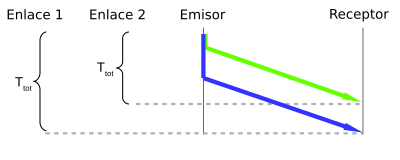
\includegraphics{img/enlaces-1.png}
\caption{Comparando enlaces de la misma longitud}
\end{figure}

En este diagrama, el tiempo total mayor corresponde al enlace 1, que es
el que tiene el mayor tiempo de transmisión.

Sin embargo, el tiempo de transmisión no es lo único que determina un
mayor tiempo de transferencia. Si los enlaces fueran de diferente
longitud, la situación podría invertirse. Un enlace de mayor velocidad
de transmisión (línea azul) podría seguir siendo el de mayor tiempo de
transferencia si fuera de longitud suficientemente mayor que el otro.

\begin{figure}[htbp]
\centering
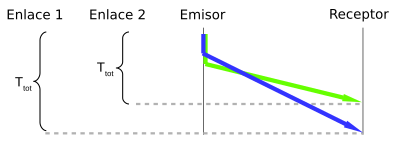
\includegraphics{img/enlaces-2.png}
\caption{Comparando enlaces de longitudes diferentes}
\end{figure}

\subsection{Entidades de red}\label{entidades-de-red}

Llamamos \textbf{entidades} a las piezas de software o de hardware que
funcionan como componentes de los nodos dentro de una red. Las entidades
pueden ubicarse a cualquier nivel: pueden ser dos routers, dos
interfaces de red, o las partes de una aplicación distribuida.

Las entidades de nodos diferentes que van a comunicarse estarán siempre
al mismo nivel.

\subsection{Eventos de red}\label{eventos-de-red}

Llamamos \textbf{eventos} a cualquier suceso de interés que ocurre
dentro de la red, especialmente si se trata de una interacción entre
entidades. Por ejemplo, la llegada de un mensaje.

\subsection{Protocolos}\label{protocolos}

Los \textbf{protocolos} son conjuntos de reglas que definen la
interacción entre dos entidades de la red.

Para comunicarse, las entidades de cualquier nivel deben compartir un
protocolo. Los protocolos especifican:

\begin{itemize}
\itemsep1pt\parskip0pt\parsep0pt
\item
  Cuál es el \textbf{formato} de los mensajes que pueden intercambiar
  las entidades;
\item
  Qué tipo de \textbf{acciones} o respuestas debe dar cada entidad al
  recibir cada mensaje.
\end{itemize}

Puede ser útil comparar los protocolos de red con protocolos sencillos
de la vida cotidiana. Muchas interacciones entre las personas están
gobernadas por protocolos, a veces poco evidentes. Por ejemplo, comprar
un artículo cualquiera en un comercio sigue unas pautas bastante
definidas.

Aunque los contenidos específicos de los mensajes pueden variar, es
habitual que existan fases en la interacción entre las personas, como el
\textbf{inicio de sesión, la autentificación, la autorización, las
peticiones o requerimientos (\emph{requests}), las respuestas
(\emph{responses}), y el cierre de sesión}.

Todas éstas son fases habituales en la comunicación entre los humanos,
pero también en los protocolos de las redes.

\subsubsection{Modelo cliente-servidor}\label{modelo-cliente-servidor}

Estas fases habituales aparecen en los protocolos que definen relaciones
de \textbf{cliente y servidor} entre entidades. En el modelo
cliente-servidor:

\begin{itemize}
\itemsep1pt\parskip0pt\parsep0pt
\item
  El nodo cliente es el que inicia una interacción, con un
  \textbf{request} o requerimiento hacia el servidor.
\item
  El nodo servidor contesta con una respuesta o \textbf{response}.
\item
  El ciclo puede repetirse indefinidamente.
\end{itemize}

La mayoría de las aplicaciones de Internet siguen este \textbf{modelo
cliente-servidor} de interacción. El protocolo \textbf{HTTP}, motor de
la \textbf{WWW}, es un ejemplo claro.

\subsubsection{Modelo peer-to-peer}\label{modelo-peer-to-peer}

El modelo cliente-servidor es asimétrico: los roles de cliente y de
servidor están bien diferenciados. Un modelo alternativo, diferente, es
el llamado \textbf{peer-to-peer}, donde no existe un nodo servidor
propiamente dicho, sino que todos los nodos que comparten el protocolo
son, a la vez, clientes y servidores, en igualdad de condiciones.

\subsubsection{Autómatas}\label{autuxf3matas}

Los \textbf{autómatas} son una herramienta formal muy útil para
describir detalladamente los protocolos. Un autómata es la
especificación de los \textbf{estados} en los que puede encontrarse una
entidad y los \textbf{eventos} que disparan los cambios de estado o
\textbf{transiciones}. El autómata puede tomar la forma de un diagrama
de burbujas y flechas.

\begin{itemize}
\item
  En un diagrama de autómata, las burbujas representan \textbf{estados}.
\item
  Las flechas representan \textbf{transiciones}.
\item
  Las flechas llevan \textbf{rótulos} que describen qué \textbf{evento}
  es necesario para disparar la transición, y qué \textbf{acción} debe
  ejecutar la entidad como respuesta al evento.

  \begin{itemize}
  \itemsep1pt\parskip0pt\parsep0pt
  \item
    Cuando no se requiere un evento para entrar en un estado (por
    ejemplo, porque es el estado inicial del autómata), el evento es
    \textbf{vacío} (y se denota ``-'').
  \item
    Un mensaje de respuesta que confirma la recepción correcta de un
    mensaje anterior se llama un \textbf{reconocimiento o
    acknowledgement (ACK)}. Si el mensaje de respuesta indica la
    \textbf{recepción incorrecta}, se llama un \textbf{acknowledgement
    negativo} o \textbf{NAK}.
  \end{itemize}
\end{itemize}

\subsubsection{Autómata del cliente}\label{autuxf3mata-del-cliente}

\begin{figure}[htbp]
\centering
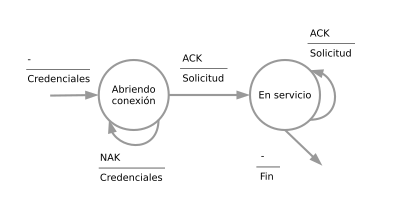
\includegraphics{img/protocolo-cliente.png}
\caption{Autómata del cliente}
\end{figure}

En el ejemplo, el cliente ingresa al estado de \textbf{Abriendo
conexión} presentando sus credenciales. Si son aceptadas, envía su
primera solicitud y pasa al estado \textbf{En servicio}. A cada
respuesta que reciba, podrá enviar una nueva solicitud. Finalmente,
emitirá un mensaje de cierre de conexión y terminará la interacción con
el servidor.

\subsubsection{Autómata del servidor}\label{autuxf3mata-del-servidor}

Por su parte, el servidor presenta un autómata complementario al del
cliente. La mayor parte del tiempo, el servidor estará en el estado
\textbf{Esperando conexión} hasta que reciba unas credenciales de un
cliente. Si las reconoce, pasa al estado \textbf{En servicio} donde
acepta solicitudes y emite respuestas. Cuando el cliente decide poner
fin a la interacción, vuelve al estado de esperar conexión de un nuevo
cliente.

\begin{figure}[htbp]
\centering
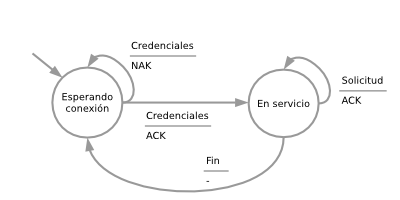
\includegraphics{img/protocolo-servidor.png}
\caption{Autómata del servidor}
\end{figure}

\subsubsection{Protocolos de parada y
espera}\label{protocolos-de-parada-y-espera}

¿Cómo se relacionan, por un lado, las medidas de tiempo de transmisión y
tiempo de propagación, y, por el otro, los autómatas de un protocolo
cliente-servidor?

Muchos protocolos requieren que una entidad reciba la confirmación de un
mensaje anterior antes de poder enviar el siguiente mensaje. Cuando esto
ocurre, decimos que el protocolo es del tipo de \textbf{parada y espera
(\emph{stop and wait})}. Cuando el enlace entre dos entidades es de
longitud muy grande, un protocolo de parada y espera puede tener una
eficiencia muy reducida.

Si la aplicación que desea usar este protocolo de parada y espera es
interactiva, y el enlace es muy largo, la experiencia de usuario será
frustrante. El usuario deberá soportar las demoras correspondientes al
tiempo de propagación de cada mensaje más el de su confirmación. Durante
ese lapso, no se puede seguir transmitiendo datos porque aún no ha
llegado la confirmación o \textbf{ACK} del mensaje anterior. Las demoras
pueden hacer que la aplicación directamente no sea viable.

El punto crucial aquí es que este problema \textbf{no se resuelve
aumentando el ancho de banda de los enlaces}, porque, como hemos dicho,
el retardo de propagación no tiene nada que ver con la velocidad de
transmisión de las interfaces.

Gran parte de la complejidad de Internet se debe a la necesidad de
resolver este problema de los protocolos de parada y espera. En
Internet, la solución está representada por el protocolo
\textbf{TCP/IP}, que en lugar de obligar a esperar un tiempo de
propagación por cada mensaje, es capaz de encadenar varios mensajes sin
necesidad de esperar confirmación por cada uno. El protocolo TCP
pertenece al nivel de \textbf{transporte} de las redes.

\textbf{Pregunta}

Supongamos que se tiene un enlace de radio de 1Gbps entre una estación
terrestre y un vehículo experimental \textbf{que circula por la
superficie de Marte}. Supongamos además que la aplicación sea controlar
interactivamente desde la Tierra este vehículo mediante un protocolo de
parada y espera. Los mensajes de este protocolo son comandos de la forma
\textbf{avanzar}, \textbf{detenerse}, \textbf{izquierda},
\textbf{derecha}, etc.

La distancia teórica mínima al planeta Marte es de unos
$54  por  10 elevado a la 6 km$. Esto se traduce en unos 3 minutos de retardo de
propagación. Quiere decir que cada comando enviado desde la Tierra a
Marte demorará, en el mejor caso, unos 6 minutos en ser confirmado. Esto
ocasiona problemas para controlar el vehículo, porque una mala maniobra
puede dejarlo en una situación peligrosa sobre el escarpado suelo
marciano. Se necesita una velocidad de respuesta mucho mayor.

Elevar el ancho de banda digital del enlace, de 1Gbps a 10Gbps, ¿sería
una solución?

\subsection{Direcciones de red}\label{direcciones-de-red}

Para poder dirigir los mensajes entre nodos, es necesario identificarlos
de alguna forma, asignándoles \textbf{direcciones} o identificadores de
red.

En Internet, las direcciones son asignadas a las interfaces, y no a los
nodos. De esta manera, si un nodo tiene más de una interfaz, recibirá
más de una dirección. El caso típico de un nodo con más de una interfaz
son los routers, que tienen una interfaz perteneciente a cada una de las
redes que conectan.

El protocolo IPv4 define las direcciones de red como números de 32 bits
que se asignan a cada interfaz de los nodos. Estas direcciones de 32
bits suelen escribirse como cuatro valores decimales, entre 0 y 255,
separados por puntos.

\textbf{Ejemplo}

\begin{itemize}
\itemsep1pt\parskip0pt\parsep0pt
\item
  La dirección IPv4 \textbf{1 1 0 0 0 0 0 0 1 0 1 0 1 0 0 0 0 0 0 0 0 0 0 1 0 0 0 0 0 0 0 1} se puede
  escribir en notación decimal con punto como \textbf{192.168.1.1}.
\end{itemize}

\subsection{Paquetes IP}\label{paquetes-ip}

Internet es una red del tipo de \textbf{conmutación por paquetes}, lo
que significa que los flujos de datos que van de un nodo emisor a un
receptor son fraccionados en \textbf{paquetes} o trozos de datos, de un
cierto tamaño máximo, y que los nodos intermedios tratan a cada paquete
individualmente para encaminarlos a su destino.

En una red conmutada por paquetes, los nodos intermedios, o routers, no
necesitan conocer todo el camino que debe atravesar cada uno de los
paquetes. En cambio, un router sólo necesita saber a cuál de los
\textbf{nodos intermedios adyacentes} encaminarlo, basándose en
información transportada por el mismo paquete.

Cada nodo intermedio o router en el camino entre el emisor y el receptor
tomará una nueva decisión de ruteo ante cada uno de los paquetes que
llegan a él.

Al generar un paquete, para que pueda ser encaminado, el emisor completa
los datos con un \textbf{encabezado} conteniendo la dirección IP del
nodo emisor, o \textbf{dirección origen}, y la dirección IP del nodo
destino, o \textbf{dirección destino}.

\subsection{Ruteo o encaminamiento}\label{ruteo-o-encaminamiento}

Cuando un paquete llega a un router, lo hace por algún enlace. La tarea
del router es \textbf{reenviar} este paquete por otro de sus enlaces, de
modo que se aproxime a su destino.

El router debe aplicar alguna regla lógica para decidir hacia qué otro
enlace \textbf{reenviar} el paquete. Esta decisión de cuál será ese otro
enlace es una acción de \textbf{ruteo} o \textbf{encaminamiento}.

\subsubsection{Tabla de reenvío o de
ruteo}\label{tabla-de-reenvuxedo-o-de-ruteo}

La decisión de ruteo es tomada por los routers usando la información de
\textbf{destino} que llevan consigo los paquetes, más información de
ruteo contenida en una \textbf{tabla de reenvío} o tabla de ruteo,
almacenada en la memoria del router.

La tabla de ruteo contiene reglas para la decisión de encaminamiento de
los paquetes. Cada regla se llama una \textbf{ruta} e indica cuál será
la interfaz de salida de los paquetes cuya dirección destino coincida
con la dirección destino de la ruta.

En líneas generales, el algoritmo de ruteo es como sigue:

\begin{itemize}
\itemsep1pt\parskip0pt\parsep0pt
\item
  Al recibir un paquete, el router examinará la dirección destino
  \textbf{del paquete} y la comparará con la dirección destino
  \textbf{de cada ruta}.
\item
  Al encontrar una coincidencia de dirección destino entre el paquete y
  la ruta, utilizará la información en la columna de \textbf{interfaz de
  salida} de esa ruta, reenviando el paquete por esa interfaz.
\end{itemize}

Sin embargo, ésta es una simplificación. La verdadera forma de la tabla
de ruteo es algo diferente. ¿Por qué?

\subsubsection{Subredes}\label{subredes}

Notemos que, ya que las direcciones IP se escriben usando 32 bits,
existen más de \textbf{cuatro mil millones} de direcciones IPv4
posibles. Una tabla de ruteo completa, con una ruta por cada dirección
destino, tal como la hemos descrito, tendría enormes requerimientos de
memoria, y el equipamiento de ruteo sería muy costoso.

Las tablas de ruteo verdaderas, entonces, no contienen una ruta por cada
dirección destino, sino que las rutas corresponden a conjuntos o
agrupaciones de direcciones, llamadas \textbf{subredes}.

Un paquete cuya dirección destino pertenezca a una subred utilizará la
ruta de dicha subred. Cualquier otra dirección destino que pertenezca a
la misma subred recibirá la misma decisión de ruteo.

Si las subredes son agrupaciones suficientemente grandes, la cantidad de
reglas de ruteo o rutas disminuirá convenientemente.

\subsubsection{Prefijo de subred}\label{prefijo-de-subred}

¿Cómo agrupar estas direcciones para definir las subredes?

\emph{Todas las direcciones con el mismo \textbf{prefijo} de una cierta
longitud formarán una subred.}

\textbf{Ejemplo}

\begin{itemize}
\item
  Las direcciones IP 130.240.10.17 y 130.240.11.15 pertenecen a una
  subred con prefijo común 130.240 de 16 bits. Todas las direcciones
  pertenecientes a esta subred se escriben como 130.240.XXX.XXX.
\item
  Sin embargo, notemos que, si escribimos las direcciones IP anteriores
  en su forma binaria, encontraremos que en realidad existe un prefijo
  común aún más largo. En efecto,

  130.240.10.17 = \textbf{1 0 0 0 0 0 1 0.1 1 1 1 0 0 0 0.0 0 0 0 1 0 1}0.0 0 0 1 0 0 0 1

  130.240.11.15 = \textbf{1 0 0 0 0 0 1 0.1 1 1 1 0 0 0 0.0 0 0 0 1 0 1}1.0 0 0 0 1 1 1 1

  Los primeros \textbf{23 bits} de ambas direcciones son iguales, luego
  comparten un prefijo común de longitud 23. Para escribirlo en notación
  decimal, adoptemos la convención de completar con ceros la parte no
  común:

  130.240.10.0 = 1 0 0 0 0 0 1 0.1 1 1 1 0 0 0 0.0 0 0 0 1 0 1 0.0 0 0 0 0 0 0 0

  Esta convención no es otra cosa que lo que llamamos la dirección de la
  subred.
\end{itemize}

\subsubsection{Dirección de subred y máscara de
subred}\label{direcciuxf3n-de-subred-y-muxe1scara-de-subred}

Cuando en una tabla de ruteo se especifique una ruta para todas las
direcciones con un mismo prefijo, la dirección destino de la ruta será
una \textbf{dirección de subred}.

Una dirección de subred se calcula utilizando una \textbf{máscara de
subred}, que es una sucesión de 32 dígitos binarios. Los primeros $n$
dígitos de la máscara son \textbf{unos}, y los restantes \textbf{ceros}.

La cantidad de dígitos ``uno'' dice cuál es la longitud del prefijo
compartido. Estos primeros $n$ dígitos ``unos'' definen cuál será el
prefijo compartido por todas las direcciones IP que pertenecen a la
subred.

\textbf{Ejemplo}

\begin{itemize}
\itemsep1pt\parskip0pt\parsep0pt
\item
  Una máscara de \textbf{24 bits} de longitud puede expresarse como
  \textbf{1 1 1 1 1 1 1 1 1 1 1 1 1 1 1 1 1 1 1 1 1 1 1 1 0 0 0 0 0 0 0 0}, que en la misma notación
  decimal de las direcciones IP suele escribirse \textbf{255.255.255.0}.
\item
  Una máscara de \textbf{26 bits} de longitud puede expresarse como
  \textbf{1 1 1 1 1 1 1 1 1 1 1 1 1 1 1 1 1 1 1 1 1 1 1 1 1 1 0 0 0 0 0 0}, o
  \textbf{255.255.255.192}.
\end{itemize}

\subsubsection{Cálculo de la dirección de
subred}\label{cuxe1lculo-de-la-direcciuxf3n-de-subred}

Para calcular la dirección de subred a la cual pertenece una dirección
IP, superponemos la dirección y su máscara de modo de encolumnar todos
los dígitos y efectuamos una operación AND bit a bit. El operador AND es
el que devuelve 1 solamente si ambos operandos son 1, y en otro caso
devuelve 0.

El efecto de este AND es \textbf{copiar} en las primeras $n$ columnas
del resultado los bits tal cual figuran en la dirección IP, y
\textbf{completar con ceros} hasta el final del resultado. Este
resultado es la dirección de subred a la cual pertenece la dirección IP
original.

\textbf{Ejemplo}

\begin{itemize}
\item
  ¿Cuál es la dirección de subred de la dirección IP
  \textbf{170.210.80.129} con máscara 255.255.255.0?

  Aplicando la máscara de 24 bits de longitud, la operación AND devuelve
  la dirección de subred \textbf{170.210.80.0}.
\item
  ¿Cuál es la dirección de subred de la dirección IP
  \textbf{170.210.80.129} con máscara 255.255.255.128?

  Si escribimos esta máscara en forma binaria, vemos que contiene
  \textbf{25 unos}. La operación AND que copia los primeros 25 bits de
  la dirección IP y deja los restantes en 0 da la dirección de subred
  \textbf{170.210.80.128}.
\end{itemize}

\textbf{Notación alternativa}

Una máscara de subred con $n$ bits suele expresarse también como
``$/n$''. Así, la dirección IP \textbf{192.168.1.1 con máscara
255.255.255.0} puede escribirse más sencillamente como
\textbf{192.168.1.1/24}.

Con los conceptos de direcciones de subred y máscaras, ya podemos
rediseñar la tabla de ruteo. Habrá que especificar \textbf{direcciones
de subred} en lugar de direcciones de hosts, y para cada ruta en la
tabla, agregar cuál es la \textbf{máscara} que define el prefijo de la
ruta.

\textbf{Nota}

Para simplificar los ejemplos siguientes, utilizaremos direcciones y
máscaras de cinco bits. Sin embargo, el mecanismo para el algoritmo de
reenvío será básicamente el mismo que con las direcciones reales IPv4 de
32 bits.

\textbf{Ejemplo}

\begin{longtable}[c]{@{}ccc@{}}
\toprule\addlinespace
Dirección de subred & Máscara & Interfaz de salida
\\\addlinespace
\midrule\endhead
0 0 0 0 0 & 1 1 1 0 0 & 0
\\\addlinespace
0 0 1 0 0 & 1 1 1 0 0 & 1
\\\addlinespace
0 0 0 1 0 & 1 1 1 1 0 & 2
\\\addlinespace
\bottomrule
\end{longtable}

Esta tabla de ruteo dice que:

\begin{itemize}
\itemsep1pt\parskip0pt\parsep0pt
\item
  La subred 0 0 0 0 0 con máscara 1 1 1 0 0 se alcanza mediante la interfaz de
  salida 0. Es decir, que si los primeros tres bits de la dirección
  destino de un paquete son 0 0 0, el paquete debe ser reenviado por la
  interfaz 0.
\item
  La subred 0 0 1 0 0 con máscara 1 1 1 0 0 se alcanza mediante la interfaz de
  salida 1. Es decir, que si los primeros tres bits de la dirección
  destino de un paquete son 0 0 1, el paquete debe ser reenviado por la
  interfaz 1.
\item
  La subred 0 0 0 1 0 con máscara 1 1 1 1 0 se alcanza mediante la interfaz de
  salida 1. Es decir, que si los primeros \textbf{cuatro} bits de la
  dirección destino de un paquete son 0 0 0 1, el paquete debe ser
  reenviado por la interfaz 2.
\end{itemize}

\textbf{Preguntas}

\begin{itemize}
\itemsep1pt\parskip0pt\parsep0pt
\item
  En el ejemplo anterior, ¿puede darse un caso donde quepa la duda de si
  aplicar la primera o la segunda regla?
\item
  ¿Puede darse un caso donde quepa la duda de si aplicar la primera o la
  tercera regla?
\end{itemize}

\subsubsection{Ruta por defecto o ruta
\emph{default}}\label{ruta-por-defecto-o-ruta-default}

Aun con la estrategia de ruteo por prefijos, los routers no pueden
conocer \textbf{todas} las rutas a todos los destinos. Siempre se apoyan
en que alguno de sus routers vecinos que esté más próximo al destino
tenga más información que ellos.

Cuando un router no sabe cómo encaminar un paquete, lo envía por una
interfaz predefinida, en la esperanza de que un router situado sobre ese
enlace, que reciba el paquete, tenga mejor información. A este router se
lo llama \textbf{router por defecto} o \textbf{gateway default}, y la
ruta que le corresponde es la \textbf{ruta por defecto o default route}.

Para definir una ruta por defecto agregamos una regla a la tabla de
ruteo con \textbf{dirección de subred = 0 0 0 0 0 y máscara de red = 0 0 0 0 0}.
Como la máscara tiene \textbf{cero unos}, cualquier dirección IP destino
da una coincidencia. Por eso, la regla por defecto se consulta en último
lugar, y como último recurso. De lo contrario, la interfaz de la ruta
por defecto absorbería todo el tráfico y nunca se reenviaría tráfico a
otros enlaces.

En Internet, tiene sentido que la interfaz de la ruta default en cada
router sea la que ``mira'' al centro de la Internet, en la dirección
donde hay más nodos. Allí es más probable que existan routers con una
configuración mejor.

\subsubsection{Rutas más específicas y máscaras más
largas}\label{rutas-muxe1s-especuxedficas-y-muxe1scaras-muxe1s-largas}

El caso de la ruta default nos permite ver que la ruta más genérica, la
menos específica, es la que tiene la máscara más corta. Representa a
cualquier subred, o al conjunto de todas las subredes.

Lo inverso también es cierto: si una máscara es más larga, la ruta es
más específica. Una máscara más larga representa una subred de
\textbf{menor} tamaño.

Una máscara larga puede servir para indicar una excepción a una regla
más general. Por eso, las máscaras más largas \textbf{tienen
preferencia} en el proceso de ruteo de un paquete.

Cada vez que un router se encuentre con más de una ruta posible, elegirá
aquella cuya máscara de subred sea más larga (es decir, \textbf{la ruta
más específica}).

\textbf{Ejemplo}

\begin{longtable}[c]{@{}ccc@{}}
\toprule\addlinespace
Dirección de subred & Máscara & Interfaz de salida
\\\addlinespace
\midrule\endhead
0 0 0 0 0 & 1 1 1 0 0 & 0
\\\addlinespace
0 0 1 0 0 & 1 1 1 0 0 & 1
\\\addlinespace
0 0 0 1 0 & 1 1 1 1 0 & 2
\\\addlinespace
\bottomrule
\end{longtable}

La primera regla indica que todo destino con sus primeros tres bits
iguales a cero se alcanza mediante la interfaz 0. Sin embargo, hay
excepciones. Los destinos que cumplan lo anterior pero tengan su
\textbf{cuarto bit} igual a 1 deben alcanzarse mediante la interfaz 2.
La tercera regla es una excepción a la primera porque trata un conjunto
más específico de direcciones.

\subsection{Algoritmo de reenvío}\label{algoritmo-de-reenvuxedo}

Finalmente podemos presentar el algoritmo de reenvío tal cual lo
ejecutan los routers de Internet.

\begin{itemize}
\itemsep1pt\parskip0pt\parsep0pt
\item
  Para cada regla en la tabla de ruteo, en orden descendente por
  longitud de prefijo

  \begin{itemize}
  \itemsep1pt\parskip0pt\parsep0pt
  \item
    Subred destino del paquete = Dirección destino del paquete AND
    Máscara de la ruta
  \item
    Si subred destino del paquete = subred de la ruta, reenviar el
    paquete por la interfaz de salida de esa ruta
  \end{itemize}
\item
  Si se agotó la tabla pero hay una ruta default

  \begin{itemize}
  \itemsep1pt\parskip0pt\parsep0pt
  \item
    Reenviar el paquete por la ruta default
  \end{itemize}
\item
  Si se agotó la tabla sin éxito

  \begin{itemize}
  \itemsep1pt\parskip0pt\parsep0pt
  \item
    Devolver error de red inalcanzable
  \end{itemize}
\end{itemize}

Como las reglas se consultan en orden de prefijos más largos a prefijos
más cortos, las rutas más específicas se encuentran primero, y tienen
preferencia sobre las menos específicas.

\textbf{Ejemplo}

Volvamos a la tabla de ruteo de un ejemplo anterior, sólo que
agregándole una ruta default por la interfaz 2:

\begin{longtable}[c]{@{}cccc@{}}
\toprule\addlinespace
Regla & Dirección de subred & Máscara & Interfaz de salida
\\\addlinespace
\midrule\endhead
1 & 0 0 0 0 0 & 1 1 1 0 0 & 0
\\\addlinespace
2 & 0 0 1 0 0 & 1 1 1 0 0 & 1
\\\addlinespace
3 & 0 0 0 1 0 & 1 1 1 1 0 & 2
\\\addlinespace
4 & 0 0 0 0 0 & 0 0 0 0 0 & 2
\\\addlinespace
\bottomrule
\end{longtable}

¿Qué camino tomarán los paquetes con la siguiente dirección destino?

\begin{itemize}
\itemsep1pt\parskip0pt\parsep0pt
\item
  0 0 0 0 1 → Interfaz 0, por la regla 1
\item
  0 0 0 1 1 → Interfaz 2, por la regla 2, ya que, a pesar de que la
  dirección destino coincide también con la regla 1, la regla 2 es más
  específica.
\item
  0 1 0 0 1 → Interfaz 2, por la regla default, ya que las anteriores no han
  resultado en coincidencias.
\end{itemize}

\subsection{Servicio de Nombres de Dominio
(DNS)}\label{servicio-de-nombres-de-dominio-dns}

Como hemos visto, el funcionamiento de Internet se basa en la existencia
de \textbf{direcciones}, que permiten enviar y encaminar el tráfico
entre los diferentes puntos de la red. Sin embargo, las direcciones IP
de 32 bits, o su equivalente de cuatro decimales con puntos, son
incómodas de manejar para los humanos. El \textbf{servicio de nombres de
dominio}, o Domain Name Service (\textbf{DNS}) es un servicio agregado a
la Internet para comodidad de los usuarios.

El servicio DNS permite a los usuarios referirse a los nodos de Internet
mediante nombres simbólicos en lugar de direcciones, y entra en acción
cada vez que se menciona el \textbf{nombre} de un nodo para hacer
contacto con él. Un nodo que necesita enviar un mensaje cualquiera a
otro nodo necesita conocer su dirección IP. Si únicamente conoce su
nombre, pedirá una \textbf{traducción de nombre} a algún
\textbf{servidor DNS}.

Técnicamente, Internet podría funcionar perfectamente (y, de hecho, lo
hizo durante algún tiempo) \textbf{sin} la existencia del servicio DNS,
pero la costumbre lo ha convertido en una parte indispensable de la red.

\subsubsection{Jerarquía de nombres de
dominio}\label{jerarquuxeda-de-nombres-de-dominio}

Estos nombres simbólicos tienen una cierta estructura jerárquica, es
decir, organizada por niveles. Un nombre consta de varias partes,
separadas por puntos. En cada nombre, las partes más a la derecha
designan conjuntos mayores de nodos, y las partes más a la izquierda,
conjuntos más pequeños, contenidos en aquellos conjuntos mayores.

\textbf{Ejemplo}

\begin{itemize}
\itemsep1pt\parskip0pt\parsep0pt
\item
  El nombre \textbf{pedco.uncoma.edu.ar} designa al nodo \textbf{pedco},
  que pertenece al conjunto \textbf{uncoma}, contenido en el conjunto
  \textbf{edu} contenido en el conjunto \textbf{ar}.
\item
  El nombre \textbf{pedco.uncoma.edu.ar} equivale, gracias al servicio
  DNS, a la \textbf{dirección IP 170.210.81.41}.
\end{itemize}

Estos conjuntos de nombres se llaman \textbf{dominios}. Los dominios que
aparecen más a la derecha son los más generales. Inicialmente fueron
siete de propósito general (\textbf{org, mil, gov, edu, com, net, int}),
más los pertenecientes a los países (\textbf{ar} para Argentina,
\textbf{cl} para Chile, \textbf{uy} para Uruguay\ldots{}), pero luego se
agregaron otros. Por ser los más generales, están al tope de la
jerarquía, y se llaman dominios de nivel superior o \textbf{TLD
(Top-Level Domains)}.

Los dominios de nivel superior contienen otros espacios de nombres,
llamados a su vez dominios, y éstos, otros llamados subdominios. En el
ejemplo anterior, el TLD es \textbf{ar}, el dominio es \textbf{edu.ar}
(educación, Argentina), el subdominio es \textbf{uncoma.edu.ar}
(Universidad del Comahue, educación, Argentina) y finalmente
\textbf{pedco.uncoma.edu.ar} es el nombre de un nodo perteneciente a la
Universidad del Comahue, educación, Argentina.

\subsubsection{Resolución de nombres}\label{resoluciuxf3n-de-nombres}

Los servidores DNS se clasifican por el tipo de función que cumplen.
Cada uno interviene de una manera especial en el mecanismo de traducción
de nombres a direcciones. Este mecanismo de traducción se llama
\textbf{resolución} de nombres.

\begin{itemize}
\item
  Cada nodo de Internet lleva una configuración que le dice cuál es la
  dirección de su \textbf{servidor DNS local}. El servidor local es
  quien responde efectivamente una consulta DNS. Normalmente, el
  servidor local se encuentra ``cerca'' del cliente en términos de
  redes. Posiblemente, en la misma red local, o en la del proveedor de
  acceso a Internet.
\item
  Al ser consultado por un nombre, un servidor local usará la estrategia
  de analizar ese nombre \textbf{de derecha a izquierda}. Utilizará los
  componentes del nombre en ese orden, es decir, yendo de lo general a
  lo particular. En primer lugar utilizará el TLD o nombre de nivel
  superior para averiguar información sobre ese conjunto de nombres.

  Los servidores locales no conocen todas las posibles traducciones de
  nombre a dirección IP, por lo cual necesitan el servicio de los
  \textbf{servidores raíz}. Estos son alrededor de una veintena de
  servidores distribuidos en diferentes lugares del planeta, y todos
  tienen la misma información, replicada: las direcciones de los
  servidores de los TLD.

  Así, un servidor local obtendrá, de un servidor raíz, el dato de dónde
  ubicar al servidor del TLD \textbf{ar}.
\item
  Conociendo la dirección IP del servidor del TLD, el servidor local lo
  interrogará entonces acerca del siguiente componente del nombre.

  Los servidores de los TLD tampoco conocen todas las posibles
  traducciones, sino que conocen las direcciones de los servidores DNS
  de los dominios por debajo de ellos. Así, el servidor del TLD
  \textbf{ar} puede decirle al servidor local dónde ubicar al servidor
  del dominio \textbf{edu.ar}.

  Otra información que este servidor del dominio TLD \textbf{ar} podría
  darle al servidor local, si la pidiera, serían las direcciones de los
  servidores de los dominios \textbf{com.ar}, \textbf{org.ar}, etc.
\item
  Ahora el servidor local puede consultar al servidor del dominio
  \textbf{edu.ar}, que es quien puede informarle la dirección del
  servidor del subdominio \textbf{uncoma.edu.ar}.
\item
  Finalmente, el servidor local consulta al servidor del subdominio
  \textbf{uncoma.edu.ar} por la traducción del nombre de nodo
  \textbf{www.uncoma.edu.ar}. Este servidor tiene en sus tablas la
  información que dice cuál es la dirección IP asignada a ese nombre.
  Ahora el servidor local puede devolver esa información al cliente que
  originalmente hizo la consulta.
\end{itemize}

Todo este complejo mecanismo debería tener lugar cada vez que un cliente
de la red consulta por un nombre. Sin embargo, como este mecanismo es
costoso en tiempo y en ancho de banda de las redes, se adopta un esquema
de \textbf{cache} o reserva de información. Como es muy probable que esa
información vuelva a ser solicitada, los pares (nombre, dirección) que
han sido resueltos quedan guardados en una memoria temporaria o
\textbf{cache} del servidor local. De esta manera las próximas consultas
podrán responderse sin necesidad de volver a generar tráfico hacia el
resto de la Internet.

\subsection{Administración de redes}\label{administraciuxf3n-de-redes}

Existen herramientas de software que permiten diagnosticar las
condiciones en que se realiza el ruteo, o encaminamiento, de los
paquetes IP. El administrador de redes las utiliza para investigar el
origen de los problemas en la red.

\subsubsection{Comando ping}\label{comando-ping}

El comando \textbf{ping} emite paquetes hacia un nodo destino. Si los
paquetes logran atravesar la Internet, el nodo destino emitirá una
respuesta. El comando ping muestra los paquetes de respuesta que llegan
o se pierden, y el tiempo que demora cada respuesta en llegar.

Cuando los usuarios tienen problemas con alguna aplicación de red, el
comando ping es útil como herramienta de diagnóstico porque permite
saber si la red es capaz de hacer llegar paquetes de un nodo a otro. Si
el diagnóstico de ping es positivo, el administrador de red no se
preocupa en comprobar cuestiones asociadas con los niveles inferiores a
la capa de red: la comunicación a nivel físico, de enlace y de red entre
ambos nodos es operativa. Si existe alguna condición de error, se deberá
a problemas relacionados con las aplicaciones, que habrá que investigar.

\subsubsection{Comando traceroute}\label{comando-traceroute}

El comando \textbf{traceroute} permite investigar cuál es la cadena
particular de routers que debe atravesar un paquete para llegar a un
destino dado. Además, da información sobre la demora en atravesar cada
enlace, lo que puede dar una idea de si existe una condición de
\textbf{congestión} en el camino de los paquetes, y en qué lugar de
Internet.

Una condición de congestión es aquella que aparece cuando los nodos
intentan utilizar un enlace más allá de su capacidad. Si un enlace es
capaz de transmitir una cantidad de bits por segundo, y las demandas de
los nodos de la red superan esa capacidad, el router comienza a acumular
o encolar paquetes hasta que no tiene más espacio en su memoria para
almacenarlos. A partir de este momento, si llegan nuevos paquetes,
simplemente los descarta. El programa traceroute hace evidentes las
pérdidas de paquetes, y dice en cuál de los enlaces ocurren.

El programa traceroute también permite detectar anomalías de ruteo como
los lazos o ciclos de ruteo, que se producen cuando los paquetes toman
caminos circulares de los cuales no pueden salir.

\end{document}
